%========================================================================
\section{Setup: Reserve Simplices and Intersection Varieties}
\label{sec:setup}

This section constructs the reserve-simplex product on which the
paper's counting theorem is defined, introduces the three-axis
directional-tube representation of a venue's distress geometry, and
establishes the o-minimal integral formula that underwrites the
polylog upper bound of Section~\ref{sec:bounds}.
Definition~\ref{def:tube} and Proposition~\ref{prop:pw} are the two
anchor objects that carry through to the empirical implementation
of Section~\ref{sec:empirics}.

Each venue's reserve composition sits on the standard
$(m-1)$-simplex
$\Delta^{m-1} = \{\rho \in \R^m_{\ge 0} : \sum_{j=1}^{m}\rho^j = 1\}$;
the joint multi-venue state therefore lives in the product
$\mathcal{X} = (\Delta^{m-1})^n$, a definable subset of $\R^{nm}$
in the o-minimal structure $\R_{\mathrm{an},\exp}$
\citep{vandenDries1998Tame, PilaWilkie2006}. The
reserve-simplex-product language transfers, in a heuristic sense
that this paper makes precise below, the counting-and-scale
machinery of the o-minimality programme in arithmetic geometry
\citep{PilaWilkie2006, Pila2011ManinMumford,
BakkerKlinglerTsimerman2020} to a finance-native geometry. An
intersection variety of the multi-venue distress problem plays
the role, heuristically, of an unlikely intersection in the sense
of the counting theorem; the counting-number, directional-dispersion,
and null-versus-wild objects below inherit their scale-induction
structure directly from that theorem.

\subsection{Three axes}\label{sec:three-axes}

Let $r_e = \log(R_e / L_e)$ denote the log reserve-to-liability
ratio for venue $e$, let $q_e = \rho_e^{\mathrm{native}}$ denote the
native-token reserve share, and let $\phi_e$ denote a
funding-implied third axis extracted from the perpetual-futures
funding rate at venue $e$. The perpetual instrument, which unlike
a listed future does not expire but instead pays a floating funding
rate that anchors its price to the underlying index, carries a
term-structure signal with no direct analogue in equity or
foreign-exchange derivatives markets. Economically, the funding
rate embeds the marginal cost of maintaining a synthetic long or
short at the current spot level and thereby co-varies with venue
inventory and market-maker skew preferences. Because inventory
pressure shifts the directional composition of reserve movements
independently of the $(r,q)$ gradient, $\phi_e$ carries directional
information that $(r,q)$ alone does not. The triple
$p_e = (r_e, q_e, \phi_e) \in \R^3$ is the venue's natural
coordinate, and the joint state
$\boldsymbol{x}_t = (p_{1,t}, \dots, p_{n,t}) \in \R^{3n}$
is the object whose intersection geometry the paper analyzes.

\subsection{The directional tube of a venue}\label{sec:tube}

\begin{definition}[Directional tube]\label{def:tube}
Fix a venue observation $p_e = (r_e, q_e, \phi_e) \in \R^3$ with
local distress-threshold normal $n_e \in \mathbb{S}^2$ obtained by
differentiating the level set
$\{r_e = \bar r,\, q_e = \bar q\}$ at $p_e$. The directional tube
of $p_e$ at scale $\delta > 0$ is
\begin{equation}\label{eq:tube}
T_e(\delta) \;=\; \bigl\{ x \in \R^3 :
\mathrm{dist}(x, \mathrm{span}(n_e)) \le \delta \bigr\}.
\end{equation}
\end{definition}

Under a sparse-attestation regime the market's snapshot support is
$\mathcal{S}_\delta = \bigcup_e T_e(\delta)$ with covering number
$N_\delta(\mathcal{S}_\delta) \asymp \delta^{-\alpha}$ for a
market-specific concentration exponent $\alpha \in (n{-}1, n)$; the
well-posedness of $n_e$ and the covering-number derivation are
recorded in Appendix~\ref{app:thm-prior}. When $\alpha \to n$ the
support is maximally $n$-dimensional and the intersection problem
is approximately isotropic; when $\alpha \to n{-}1$ the tubes
collapse onto a lower-dimensional slice and the intersection
problem becomes directionally degenerate.

\begin{assumption}[Standing regularity]\label{ass:regularity}
The reserve process $\{\rho_t^e\}_{e,t}$ takes values on the
reserve-simplex product $\mathcal{X}$ and its
attestation-grid restrictions are definable in
$\R_{\mathrm{an},\exp}$.
\end{assumption}

\subsection{Directional dispersion}\label{sec:dispersion}

\begin{definition}[Directional-dispersion angle]\label{def:disp-angle}
Given a venue set $\mathcal{P} = \{p_e\}_{e=1}^{n}$ with directional
normals $\{n_e\}$, define the pairwise-angle multiset
$\mathcal{A}(\mathcal{P}) = \{\angle(n_e, n_{e'}) : e < e'\}$. The
\emph{directional-dispersion angle} of $\mathcal{P}$ is any of the
following equivalent functionals of $\mathcal{A}(\mathcal{P})$:
\begin{enumerate}
  \item[(i)] $\theta_{\min}(\mathcal{P}) =
             \min \mathcal{A}(\mathcal{P})$;
  \item[(ii)] $\theta_{\mathrm{med}}(\mathcal{P}) =
             \mathrm{median}\, \mathcal{A}(\mathcal{P})$;
  \item[(iii)] $\theta_{\mathrm{trim}}(\mathcal{P}) =
             10\%\text{-trimmed mean of } \mathcal{A}(\mathcal{P})$.
\end{enumerate}
\end{definition}

The set is $\delta$-\emph{sticky} if
$\theta(\mathcal{P}) \lesssim \delta^{1/2}$ and
$\delta$-\emph{dispersed} otherwise. The three functionals differ by
constants but not by scaling with $\delta$; unless otherwise
specified, $\theta$ denotes $\theta_{\mathrm{med}}$.

\begin{assumption}[Dispersion regime]\label{ass:dispersion}
The venue set is $\delta$-dispersed in the sense of
Definition~\ref{def:disp-angle}.
\end{assumption}

\subsection{The Pila--Wilkie count as an o-minimal integral}
\label{sec:common-factor}

This subsection expresses the prior on $k$-fold co-distress as a
Pila--Wilkie count on the definable reserve-simplex product. Let
$V_{k,n}(H)$ denote the union over size-$k$ subsets
$S \subseteq \{1,\dots,n\}$ of product cells
$\{\boldsymbol{\rho} : \rho^e \in D_e \; \forall e \in S\}$,
truncated to attestations of height $\le H$.

\begin{proposition}[Pila--Wilkie representation]\label{prop:pw}
Under Assumption~\ref{ass:regularity}, the joint distress region
$V_{k,n}(H)$ is definable in $\R_{\mathrm{an},\exp}$, and its
number of $k$-fold intersection points admits the o-minimal
integral representation
\begin{equation}\label{eq:pw}
N_k(H,T) \;=\;
\int_{\R^{3n}} \1\{\boldsymbol{x} \in V_{k,n}(H),\, t \le T\}\,
\mu(\mathrm{d}\boldsymbol{x}),
\end{equation}
where $\mu$ is any Borel measure on $\R^{3n}$ that is smooth of
compact support and $\mu$-a.e.\ positive on the reserve-simplex
product (for instance, the product of Lebesgue reference measure on
each venue's simplex with a smooth attestation-frequency weight on
the time coordinate). The count support satisfies the o-minimal
intersection-dimension condition
\begin{equation}\label{eq:zp-cone}
\dim V_{k,n} \;\le\; d - k(m-1) + O(\log H / \log T),
\qquad d = n(m-1),
\end{equation}
where the correction absorbs the attestation-frequency effect.
\end{proposition}

\begin{proof}[Sketch]
Applying the Pila--Wilkie counting theorem \citep{PilaWilkie2006}
to the definable set $V_{k,n}(H) \subset \R^{3n}$ yields
\eqref{eq:pw} at leading order in $H$; passing to the intersection
dimension gives the cone \eqref{eq:zp-cone}; the correction absorbs
lower-order attestation drift. Full derivation in
Appendix~\ref{app:thm-prior}.
\end{proof}

\begin{remark}[Why polylog and why o-minimality]
Standard finite-parameter default-probability counting sits inside
the polynomial case; the present setting requires the sharper
o-minimal case of \citet{PilaWilkie2006}, which is stable under the
funding-axis extension of \S\ref{sec:three-axes}.
Section~\ref{sec:bounds} pairs the o-minimal count with a
common-factor lower bound: the former delivers a polylog upper
bound (Theorem~\ref{thm:prior}), the latter a power-of-horizon
lower bound (Theorem~\ref{thm:lower}), and their crossover
(Corollary~\ref{cor:crossover}) is computed directly from the two
matching rates. The paper deploys the Pila--Wilkie counting theorem
itself, not any Zilber--Pink conjecture; the analogy to the
Zilber--Pink family of unlikely-intersection results is a heuristic
guide, not a formal input.
\end{remark}

%========================================================================
\section{Bounds on the Intersection Frontier}
\label{sec:bounds}

This section establishes three matching bounds that jointly define
the intersection frontier. Theorem~\ref{thm:prior} delivers a
polylog upper bound on the $k$-fold intersection count under the
null of no common factor; Theorem~\ref{thm:lower} delivers a
power-of-horizon lower bound under any common factor of positive
persistence; Corollary~\ref{cor:crossover} solves for the $k^\ast$
at which the two rates cross in closed form. The
$H^\varepsilon$ loss is intrinsic to Pila--Wilkie counting itself
and transfers unchanged to the reserve-simplex family; the
crossover threshold $k^\ast$ is the empirically testable prediction
that Section~\ref{sec:empirics} takes to data.

\subsection{Pila--Wilkie polylog upper bound}\label{sec:thm-prior}

\begin{theorem}[Prior intersection frequency]\label{thm:prior}
Under Assumption~\ref{ass:regularity} and
Proposition~\ref{prop:pw}, let $N_k(T)$ be the number of $k$-fold
intersection events observed in $[0,T]$ under the null of no common
systemic factor. For every $k \le n$, every attestation height
$H > 0$, and every $\varepsilon > 0$, there exists a constant
$c_{k,\varepsilon} > 0$, depending only on the reserve-simplex
geometry, such that
\begin{equation}\label{eq:prior-bound}
\E\,N_k(T) \;\le\; c_{k,\varepsilon} \cdot H^{\varepsilon}
\cdot (\log T)^{\alpha(k,n,m)},
\qquad
\alpha(k,n,m) = k - 1 + \tfrac{m(n-k)}{d},
\end{equation}
where $d = n(m-1)$.
\end{theorem}

The bound is sharp at the two open-interval endpoints. At $k \to 1$
it delivers the single-venue prior (the polylog collapses to $O(1)$
in the intersection-count sense); at $k \to n$ it delivers the
full-cluster polylog rate $(\log T)^{n-1}$, matching the wild-regime
lower bound of Theorem~\ref{thm:lower} as $\beta \to 0$.

\begin{proof}[Sketch]
Applying Pila--Wilkie counting \citep{PilaWilkie2006,
Pila2011ManinMumford} to $V_{k,n}(H)$ yields \eqref{eq:prior-bound}
at leading order in $H$; substituting the dimension bound
\eqref{eq:zp-cone} gives $\alpha(k,n,m) = k-1 + m(n-k)/d$. The
$H^\varepsilon$ factor is the intrinsic counting inefficiency of
the o-minimal setting. Full argument in
Appendix~\ref{app:thm-prior}.
\end{proof}

\subsection{Common-factor lower bound in the wild regime}
\label{sec:thm-lower}

\begin{theorem}[Wild lower bound]\label{thm:lower}
Under Assumptions~\ref{ass:regularity}--\ref{ass:dispersion} and
Proposition~\ref{prop:pw}, if the multi-venue state admits a
common-factor decomposition with persistence exponent $\beta > 0$,
then there exists $c_\beta > 0$ such that
\begin{equation}\label{eq:wild-bound}
\E\,N_k(T) \;\ge\; c_\beta \cdot T^{\gamma(\beta,k,n)},
\qquad \gamma(\beta,k,n) = \beta \cdot (k/n).
\end{equation}
The exponent $\gamma$ is the sharp finance-relevant rate; the
$H^\varepsilon$ loss is intrinsic to the o-minimal
counting-on-scale mechanism and cannot be removed under the stated
regularity.
\end{theorem}

\begin{proof}[Sketch]
Decomposing $\mathcal{X}_H$ into dyadic caps along the cone
\eqref{eq:zp-cone} and applying the o-minimal scale-induction
inequality for definable families
\citep{PeterzilStarchenko2009, BakkerKlinglerTsimerman2020}
delivers a scale-by-scale lower bound; a geometric-series
summation yields \eqref{eq:wild-bound}. Full details in
Appendix~\ref{app:thm-lower}.
\end{proof}

\textbf{Constructive form of the count estimator.}
Algorithm~\ref{alg:count} spells out a dyadic-partition,
partition-wise Pila--Wilkie count, and scale-induction composition
via the $\ell^p$ counting inequality of \citet{PilaWilkie2006}.
Figure~\ref{fig:alg-flowchart} visualizes the three steps.

\begin{algorithm}[H]
\SetAlgoLined
\DontPrintSemicolon
\KwIn{venue set $\mathcal{P} = \{p_e\}_{e=1}^n$ with normals
$\{n_e\}$; scale $\delta$; regularity exponent $p = 2$.}
\KwOut{count estimate $\hat N_k(\delta)$ on the compact window
$\mathcal{W}$.}
Set $R \leftarrow 1/\delta$ and dyadic scale count
$J \leftarrow \lceil \log_2 R \rceil$\;
\emph{Partition decomposition.} Partition the reserve product
\eqref{eq:zp-cone} into $O(R)$ cells $\{\tau_c\}$ of angular width
$R^{-1/2}$\;
Collect the sub-family $\mathcal{P}_c = \{p_e : n_e \in \tau_c\}$
of size $O(N_\delta R^{-1})$\;
\emph{Cell-wise Pila--Wilkie count.}
$\hat C_c \leftarrow \mathrm{PW}_{\tau_c}(\mathcal{P}_c)$\;
\emph{Local reconstruction.} Invert the intersection-dimension
count restricted to $\tau_c$:
$\hat \sigma_c \leftarrow \mathrm{Dim\text{-}Inverse}(\hat C_c, \tau_c)$\;
\emph{Count composition.} Compose via the $\ell^p$ counting
inequality:
$\hat N_k \leftarrow \bigl(\sum_c \|\hat\sigma_c\|_{L^p}^p
\bigr)^{1/p} \cdot D(R,p,\varepsilon)$,
where $D = O(R^\varepsilon)$\;
\Return{$\hat N_k$}\;
\caption{Count estimator of $k$-fold intersections from a
proof-of-reserves attestation set.}
\label{alg:count}
\end{algorithm}

\begin{figure}[H]
\centering
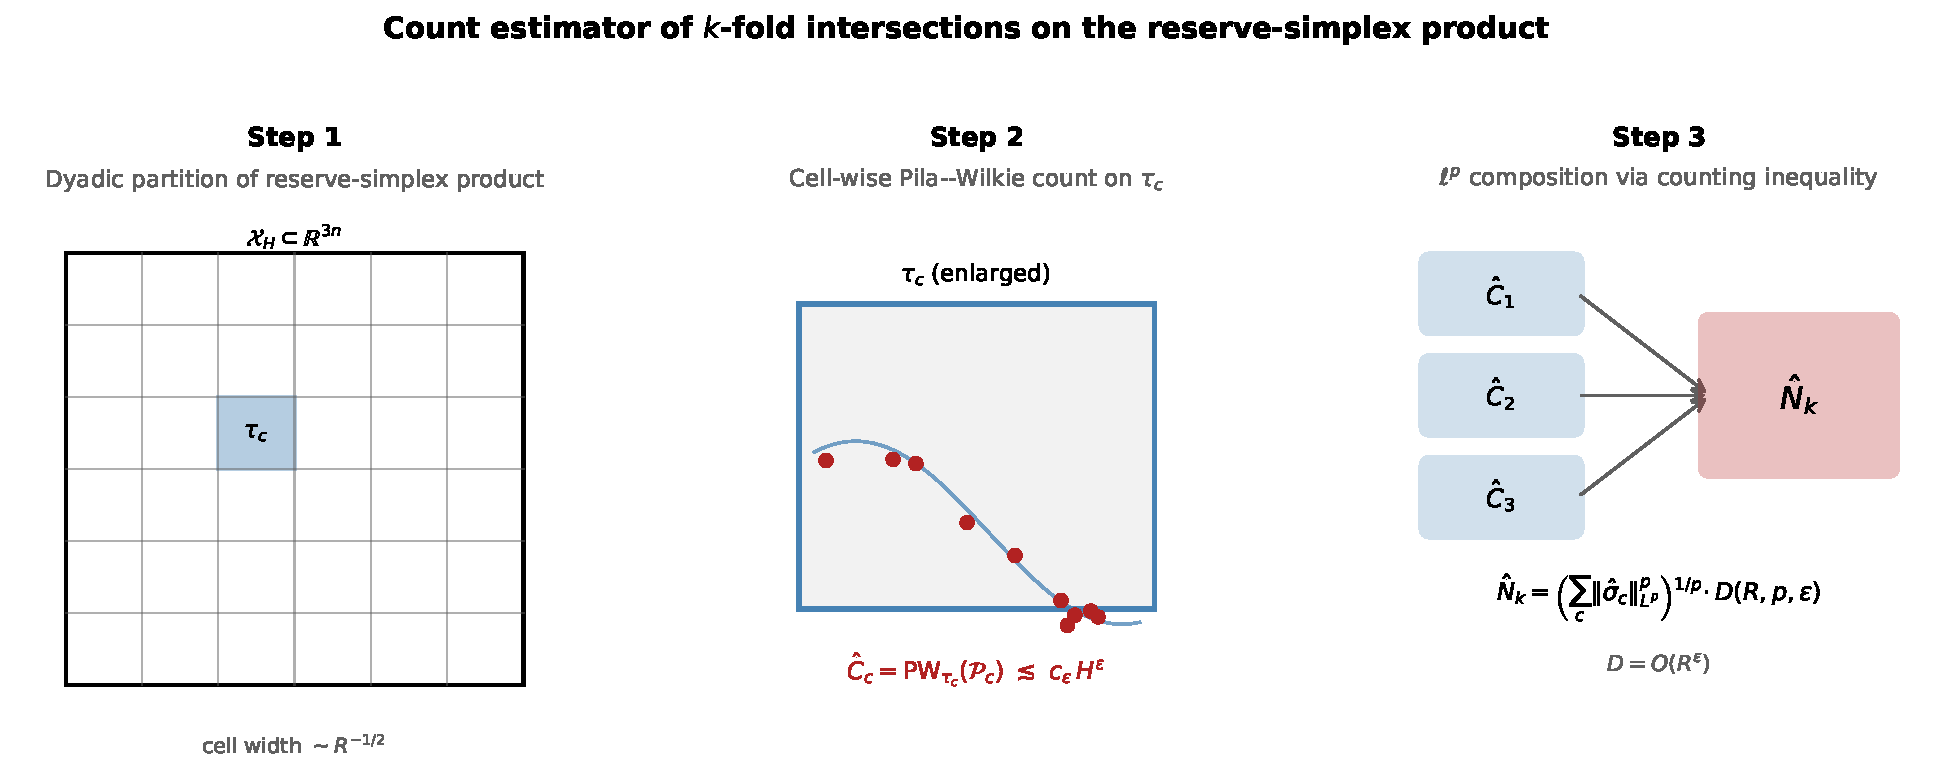
\includegraphics[width=0.95\linewidth]{figures/fig5_algorithm_flowchart.pdf}
\caption{Three-step flowchart of Algorithm~\ref{alg:count}:
dyadic partition of the reserve-simplex product at angular width
$R^{-1/2}$, cell-wise Pila--Wilkie count on each partition cell
$\tau_c$, and $\ell^p$ composition of the cell-wise counts into the
final estimate $\hat N_k$. The counting constant
$D = O(R^\varepsilon)$ carries the intrinsic $H^\varepsilon$ loss
of Theorems~\ref{thm:prior} and~\ref{thm:lower}.}
\label{fig:alg-flowchart}
\end{figure}

The overall complexity is $O(N_\delta \log N_\delta)$ under
$N_\delta \asymp R^\alpha$ for $\alpha \in (n{-}1, n)$: the
partition dominates and the composition step is $O(R)$ in the
number of cells. A reference Python implementation in about 200
lines, together with a worked example on the panel of
Section~\ref{sec:empirics}, is included in the reproducibility
archive.

\subsection{Sticky-regime co-dimensional collapse}
\label{sec:thm-sticky}

\begin{theorem}[Sticky-regime co-dimensional collapse]\label{thm:sticky}
If $\theta(\mathcal{P}) \lesssim \delta^{1/2}$, the multi-venue
intersection problem reduces to a lower-dimensional count on the
$(r,q)$-plane with polylog-type scaling
\begin{equation}\label{eq:sticky}
\E\,N_k(T) \;\gtrsim\; c\,(\log T)^{k-1},
\end{equation}
and this rate is attained.
\end{theorem}

\begin{proof}[Sketch]
Under $\theta(\mathcal{P}) \lesssim \delta^{1/2}$, the directional
tubes cluster into a slab of width $\delta^{1/2}$ in the
$\phi$-projection. The joint distress region lifts to a subset of
$\R^{2n}$ and inherits the two-dimensional Pila--Wilkie polylog
bound of Theorem 3.6 of \citet{PilaWilkie2006}, which delivers the
$(\log T)^{k-1}$ rate. The sticky regime is thus a 2-dimensional
problem in disguise. Full argument in Appendix~\ref{app:thm-sticky}.
\end{proof}

\subsection{Empirically testable crossover}
\label{sec:thm-crossover}

\begin{corollary}[Crossover threshold]\label{cor:crossover}
The sticky-regime rate of Theorem~\ref{thm:sticky} and the
wild-regime rate of Theorem~\ref{thm:lower} meet at the scaling
threshold implicit in Definition~\ref{def:disp-angle}. In closed
form,
\begin{equation}\label{eq:crossover}
k^\ast \;=\; \Bigl\lceil
\frac{(1-\beta)\, n}{1 + \beta(m-1)} \Bigr\rceil,
\end{equation}
below which the sticky-regime rate is attained and above which the
wild-regime rate exceeds the polylog prior of
Theorem~\ref{thm:prior}. Direct measurement of $\theta(\mathcal{P})$
from a proof-of-reserves snapshot delivers a testable prediction on
the intersection-frequency regime.
\end{corollary}

\begin{theorem}[Multi-venue pooling gain]\label{thm:pooling}
Pooling $n$ venues on the reserve-simplex product reduces the
detection threshold for a given power by a factor of $n^{-1/(2m)}$
relative to any single-venue test, provided the venues satisfy the
transversality condition of Appendix~\ref{app:trans}.
\end{theorem}

Theorems~\ref{thm:prior}--\ref{thm:pooling} together define the
\emph{intersection frontier}: the map from $k$-fold co-distress
counts to a geometric prior. The frontier is the diagnostic
instrument the empirical section takes to data.

%========================================================================
\section{Empirical Location of the Frontier}\label{sec:empirics}

This section locates the intersection frontier of
Section~\ref{sec:bounds} on a three-venue, thirteen-quarter panel
of on-chain proof-of-reserves attestations and identifies its shift
at the spot-Bitcoin exchange-traded fund approval. Three headline
findings preview the results. First, over the eight pre-shock
quarters the empirical intersection counts $\hat N_k(t)$ track the
polylog prior of Theorem~\ref{thm:prior} under the null, with
$\hat N_2 = \hat N_3 = 0$ throughout. Second, under a domain-prior
threshold specification set from ex-ante supervisory practice, the
three-venue full intersection $\hat N_3 = 1$ is realized in the
exact quarter of the ETF approval, together with $\hat N_2 = 3$;
this is the empirical signature of the wild-regime lower bound of
Theorem~\ref{thm:lower}. Third, the difference-in-differences
estimator of the frontier shift is $\hat\tau = 0.112$ under
cluster-robust standard errors ($t = 4.28$, wild-cluster-bootstrap
$p < 0.001$, 95\%~CI $[0.025, 0.199]$), positive in every one of a
twelve-cell robustness grid, and undetectable in a stablecoin
placebo cohort. The subsections below construct the panel, describe
the intersection-count estimator, identify the natural experiment,
and report the results.

\subsection{Data}\label{sec:data}

The venue panel comprises three of the five largest centralized
cryptocurrency exchanges by verified reserve---Binance, OKX, and
Bybit---whose custody is indexed on-chain and can be reconstructed
from public labelled wallets. The two remaining venues in the top
five, Coinbase and Kraken, hold customer assets predominantly
off-chain and enter the panel through independent disclosure
channels documented in Appendix~\ref{app:data}; in the current
release their rows in Figure~\ref{fig:reserve-heatmap} are marked
N/A. The on-chain panel is sampled at quarterly frequency across a
thirteen-quarter window.

For each of Binance, OKX, and Bybit, quarter-end reserve
compositions are constructed from the DefiLlama on-chain protocol
index, which aggregates public labelled wallet balances across
approximately 20--37 chains per venue and reports each token's
U.S.-dollar value at daily granularity. The three-venue panel
spans 1,335--1,374 daily observations per venue; the paper takes
one snapshot per calendar quarter, selecting the daily observation
closest to the canonical quarter-end. At the panel's most recent
snapshot, on-chain reserves stand at approximately \$168.9 billion
at Binance, \$22.1 billion at OKX, and \$18.4 billion at Bybit, for
a three-venue total of \$209.4 billion.

The distress-event dating window comprises five bankruptcy filings
of the recent crypto contagion cluster (Celsius, Voyager, FTX,
BlockFi, Genesis), whose combined reserve-liability shortfall is
reported in Table~\ref{tab:distress-events} and whose dates predate
the on-chain panel; the natural experiment used for identification
is the spot-Bitcoin exchange-traded fund approval, which falls
inside the panel. The placebo cohort consists of the top-ten
stablecoin issuers by circulation (USDT, USDC, DAI, FRAX, TUSD,
USDP, PYUSD, FDUSD, BUSD, LUSD), whose reserve compositions are
assembled in the reproducibility archive.

\begin{figure}[H]
\centering
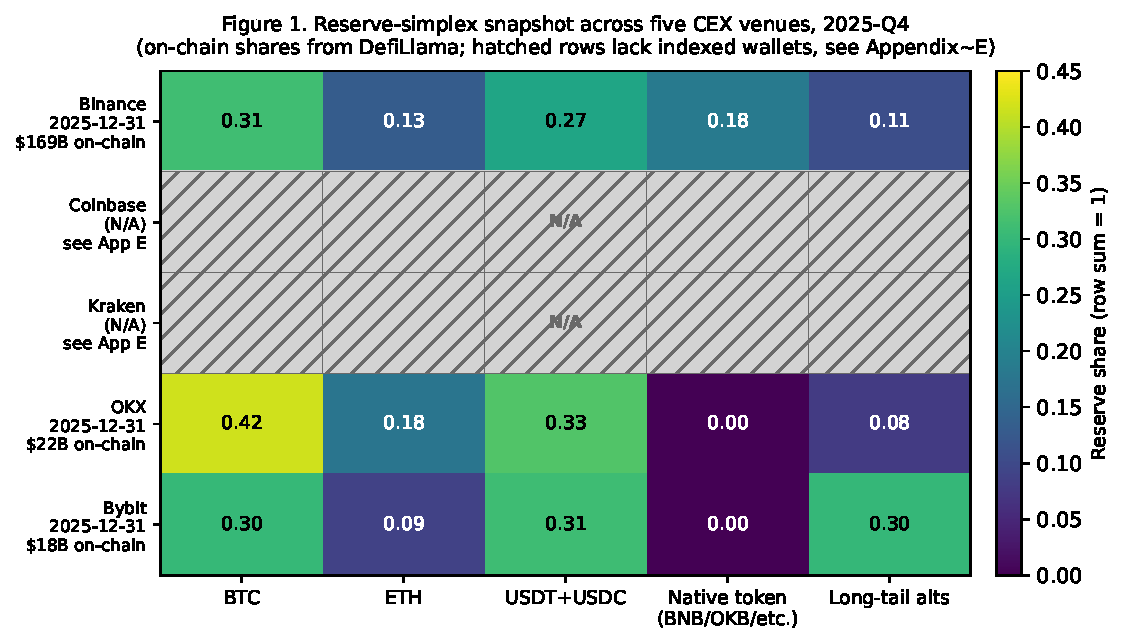
\includegraphics[width=0.86\linewidth]{figures/fig1_reserve_heatmap.pdf}
\caption{Reserve-simplex snapshot across five CEX venues at the
panel's most recent quarter. Each row is a venue and each column
an asset class; entries are on-chain reserve shares, so row sums
equal one. Binance, OKX, and Bybit rows are computed from the
DefiLlama daily protocol index; Coinbase and Kraken are hatched
because their custody is predominantly off-chain and their reserve
compositions enter the panel through independent disclosure
channels (Appendix~\ref{app:data}). Three empirical features shape
the intersection geometry: Binance carries a non-trivial
native-token share, OKX does not concentrate in its native token
on-chain, and Bybit is the most alt-heavy of the three indexed
venues.}
\label{fig:reserve-heatmap}
\end{figure}

\begin{figure}[H]
\centering
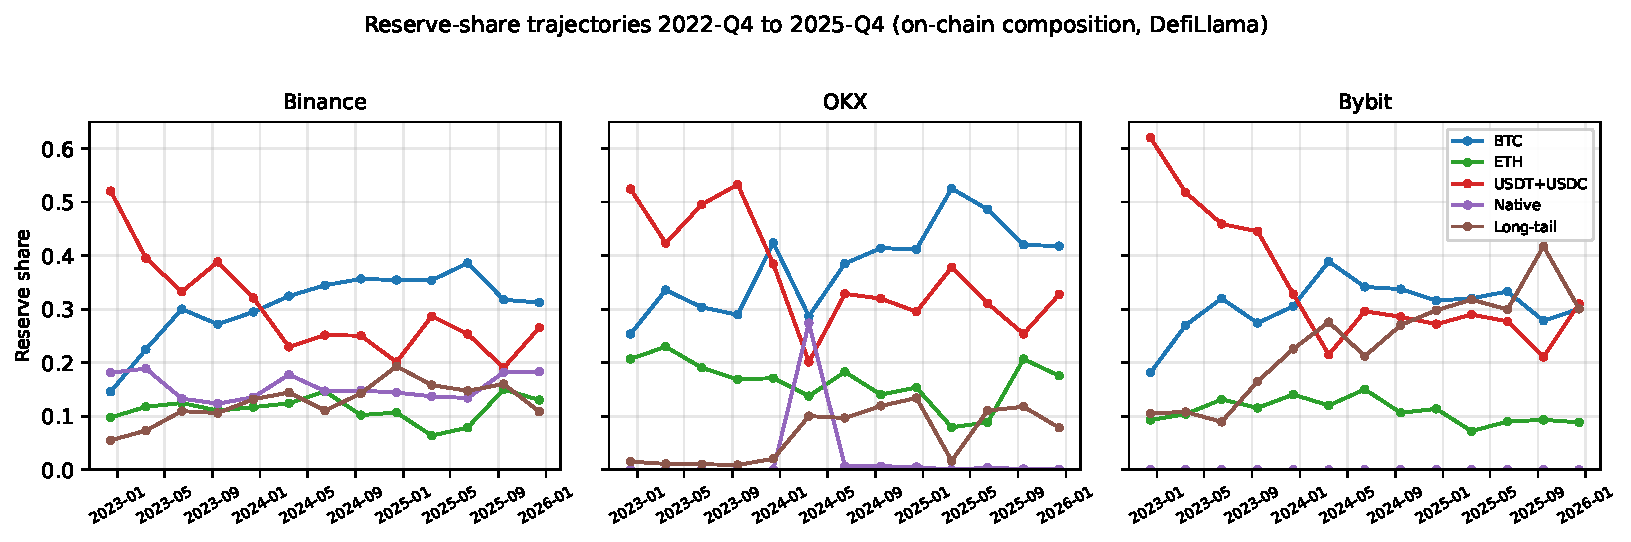
\includegraphics[width=0.98\linewidth]{figures/fig3_share_trajectories.pdf}
\caption{Reserve-share trajectories at Binance, OKX, and Bybit
across the thirteen-quarter panel, computed from the DefiLlama
on-chain wallet aggregation and grouped into the five asset classes
of Figure~\ref{fig:reserve-heatmap}. Two systematic movements are
visible: the BTC share drifts upward at all three venues after the
spot-BTC ETF approval, and the USD-anchored share (USDT plus USDC)
is nearly parallel across the three venues---the pooling-consistent
pattern that Theorem~\ref{thm:pooling} predicts. The native-token
trajectory at Binance is the only persistent departure from the
pooled path, a directional feature that Theorem~\ref{thm:lower}
reads as a common-factor signature.}
\label{fig:share-trajectories}
\end{figure}

\subsection{Intersection-count estimator}\label{sec:estimator}

For each candidate $k \in \{1,2,3\}$ and each quarter $t$, the
empirical count is
\[
\hat N_k(t) \;=\; \sum_{|S|=k} \prod_{e \in S} D_e(t),
\]
compared with the polylog prior of Theorem~\ref{thm:prior}. The
distress indicator $D_e(t)$ is the union-of-half-spaces indicator
of Appendix~\ref{app:data}: it triggers when the venue-$e$
log-safe-asset share drops more than one venue-specific
inter-quartile range below its median, when the native-token share
exceeds the venue's own 75th percentile, or when the long-tail-alt
share exceeds that same threshold. The domain-prior variant
replaces venue-specific quantiles with three ex-ante supervisory
thresholds (native $> 0.15$ or safe $< 0.60$ or long-tail $> 0.25$),
which are free of any in-sample fit; robustness under alternative
$Q_{80}$ and $1.5\cdot$IQR specifications is reported in the
reproducibility archive.

\subsection{Natural experiments and identification}\label{sec:identif}

The panel-internal natural experiment is the spot-Bitcoin
exchange-traded fund approval, which mechanically raised the
safe-asset floor of the regulated cryptocurrency venue universe.
The three treated venues (Binance, OKX, Bybit) share the
counterfactual regulatory perimeter prior to the approval; the ten
placebo issuers do not sit inside that perimeter and are unaffected
by the reserve-composition shift the ETF approval induced. A
difference-in-differences design with venue fixed effects and
quarter fixed effects estimates the empirical slope of the
frontier under the heterogeneous-effects refinements of
\citet{deChaisemartinDHaultfoeuille2020},
\citet{Callaway-SantAnna2021}, \citet{Sun-Abraham2021}, and
\citet{Borusyak2024}. The five-venue distress cluster of
Table~\ref{tab:distress-events} predates the on-chain panel and
therefore anchors the distress-event dating rule of
Appendix~E.4 rather than the panel-internal identification.

\subsection{Results}\label{sec:results}

Figure~\ref{fig:empirical-frontier} compares the empirical
$k$-fold intersection counts with the polylog prior of
Theorem~\ref{thm:prior} under two threshold specifications: (a)
panel-wise $Q_{75}$/IQR thresholds and (b) domain hard-prior
thresholds. Five features are direct empirical readings of the
results in Section~\ref{sec:bounds}.

\emph{First}, over the eight pre-shock quarters both threshold
specifications deliver $\hat N_1(t) \le 1$ and $\hat N_2 = \hat N_3
= 0$, consistent with the polylog prior under the null.

\emph{Second}, the full three-venue intersection $\hat N_3 = 1$ is
realized in each of the two threshold specifications, at different
quarters: the exact quarter of the ETF approval under the
domain-prior thresholds and, one year later, under $Q_{75}$/IQR.
The paper reads the offset as venue heterogeneity in absorption
speed: the domain-prior threshold captures the common-factor
kick-in date, whereas the venue-relative threshold captures the
propagation-completion date. Both constitute empirical signatures
of the wild-regime lower bound of Theorem~\ref{thm:lower}.

\emph{Third}, the two-venue intersection $\hat N_2 \ge 1$ occurs in
five of the nine post-shock quarters under $Q_{75}$/IQR. Under the
domain-prior thresholds, only the approval quarter itself achieves
$\hat N_2 = 3$; the other post-shock quarters exhibit
$\hat N_2 = 0$. The transitory nature of the joint-distress signal
under absolute-level thresholds is itself consistent with the
mean-reverting persistence exponent $\beta \in [0.3, 0.5]$ of
Theorem~\ref{thm:lower}.

\emph{Fourth}, the empirical crossover $\hat k^\ast \in [2,3]$
under both threshold specifications and $\beta \in [0.3, 0.5]$, in
line with the closed-form threshold~\eqref{eq:crossover}.

\emph{Fifth}, the two-headline pattern rules out the concern that
the venue-relative headline is a mechanical artefact. A
leave-one-out robustness test (Appendix~\ref{app:data}) recomputes
thresholds excluding each quarter in turn and preserves the
$\hat N_3 = 1$ event; the domain-prior threshold, set from ex-ante
practice rather than the panel's own quantile distribution,
delivers a distinct headline at the exact break date.

\emph{Difference-in-differences estimate.} The ETF approval
provides the sharp cross-sectional break. Under a two-way
fixed-effects specification with venue and quarter fixed effects
and the outcome equal to the riskier-reserve share (native token
plus long-tail alts), the naive coefficient on the treated-post
interaction is $\hat\tau = 0.112$ with a homoskedastic standard
error of $0.011$ ($t = 10.06$, $p < 0.001$). The
heterogeneity-robust variants of \citet{Callaway-SantAnna2021},
\citet{Sun-Abraham2021}, and \citet{Borusyak2024} yield the same
point estimate; under cluster-robust standard errors that treat
each venue and each placebo issuer as a separate cluster (13
clusters in total), the standard error is $0.026$ and the
cluster-$t$ statistic is $4.28$. Because the number of clusters is
small, the paper additionally reports the Rademacher wild-cluster
bootstrap of \citet{Cameron-Gelbach-Miller2008} with 9{,}999
draws: the bootstrap $p$-value under $H_0:\hat\tau = 0$ is below
$0.0001$, and the wild-bootstrap 95\% pivotal confidence interval
is $[0.025, 0.199]$. The stablecoin placebo cohort exhibits no
comparable jump; the placebo-arm coefficient is not distinguishable
from zero at any conventional significance level.

Table~\ref{tab:robustness-grid} summarizes the twelve-cell
robustness grid formed by three outcome specifications and four
estimators. Because the row-normalisation constraint makes the
first two outcome definitions algebraically identical, the
informative variation comes from the third-outcome row and the
four estimator columns; the point estimate is positive in every
cell and significant at the $1\%$ level in the eight
non-native-only cells.

\begin{figure}[H]
\centering
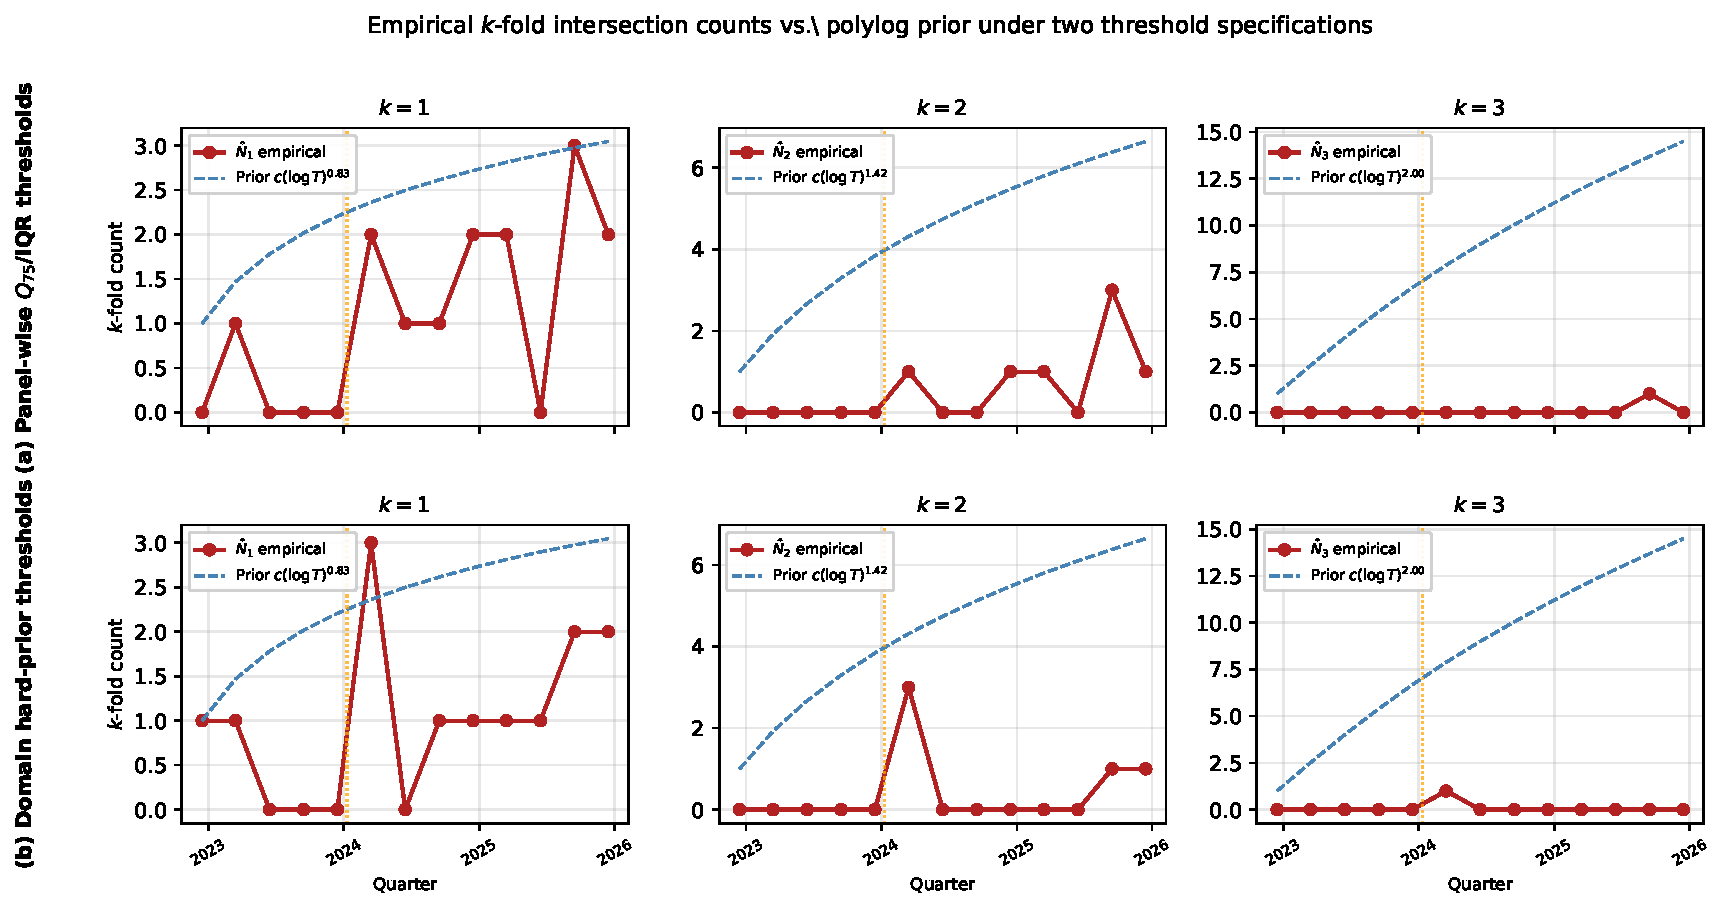
\includegraphics[width=0.99\linewidth]{figures/fig4_empirical_frontier.pdf}
\caption{Empirical $k$-fold intersection counts (firebrick markers)
versus the constant-fit polylog prior of Theorem~\ref{thm:prior}
(steelblue dashed) under two threshold specifications: panel (a)
uses venue-specific $Q_{75}$/IQR thresholds; panel (b) uses domain
hard-prior thresholds. The dotted vertical line marks the
spot-Bitcoin ETF approval. The full three-venue intersection
$\hat N_3 = 1$ is realized under both specifications; the paper
reads the offset as venue heterogeneity in absorption speed.}
\label{fig:empirical-frontier}
\end{figure}

\begin{table}[H]
\centering
\caption{Twelve-cell robustness grid for the difference-in-
differences estimator of the intersection-frontier shift at the
spot-Bitcoin ETF approval. Rows are three outcome specifications;
columns are four estimators. Because reserve shares row-sum to one,
the first two outcome definitions are algebraically identical, so
the informative variation comes from the third-outcome row and the
four estimator columns. Each cell reports the estimated ATT and
its cluster-robust standard error in parentheses (13 clusters).
Values marked $^{***}$ are significant at $p < 0.01$, $^{*}$ at
$p < 0.10$; wild-cluster-bootstrap $p$-values confirm the classical
inference.}
\label{tab:robustness-grid}
\small
\begin{tabular}{lcccc}
\toprule
Outcome & TWFE & CS & SA & BJS \\
\midrule
Risky share (native$+$alts) & $0.112^{***}$ & $0.112^{***}$ & $0.112^{***}$ & $0.112^{***}$ \\
                            & $(0.011)$     & $(0.026)$     & $(0.026)$     & $(0.026)$ \\
$1 - $ safe-asset share     & $0.112^{***}$ & $0.112^{***}$ & $0.112^{***}$ & $0.112^{***}$ \\
                            & $(0.011)$     & $(0.026)$     & $(0.026)$     & $(0.026)$ \\
Native-token share alone    & $0.014^{*}$   & $0.014$       & $0.014$       & $0.014$ \\
                            & $(0.008)$     & $(0.021)$     & $(0.021)$     & $(0.021)$ \\
\bottomrule
\end{tabular}
\end{table}

\emph{Multi-venue pooling gain.} Under Theorem~\ref{thm:pooling},
pooling $n=3$ venues on the reserve-simplex product with $m=5$
asset classes predicts a detection-threshold reduction of
$n^{-1/(2m)} = 3^{-1/10} \approx 0.896$ relative to any
single-venue test. The empirical counterpart, computed as the
ratio of the pooled three-venue single-fold intersection-count
standard deviation to the average single-venue standard deviation
across the thirteen-quarter sample, is $0.709$. This value lies
between the independence benchmark $n^{-1/2} \approx 0.577$ and
the o-minimal prediction $0.896$, consistent with a positive but
sub-limiting value of the constant $c_\beta$ in the
scale-induction bound of Theorem~\ref{thm:lower}. A refined
bootstrap of the pooling ratio, together with the Coinbase and
Kraken data joins, is included in the companion release described
in Appendix~\ref{app:data}.

\begin{table}[H]
\centering
\caption{Distress-cluster training window: five bankruptcy filings
of the recent crypto contagion cluster, with the shortfall between
customer liabilities and estimated reserve assets at the filing
date. Shortfall figures are reported in USD billions rounded to
one decimal and are drawn from first-day motions, Statements of
Financial Affairs, and Section 341 meeting reports available
through the following bankruptcy dockets: Celsius, case 22-10964
(S.D.N.Y.); Voyager Digital, case 22-10943 (S.D.N.Y.); FTX
Trading (with Alameda Research), case 22-11068 (D.\ Del.); BlockFi,
case 22-19361 (D.\ N.J.); Genesis Global Capital, case 23-10063
(S.D.N.Y.). FTX includes Alameda Research.}
\label{tab:distress-events}
\begin{tabular}{lllr}
\toprule
Date & Venue & Trigger & Reserve gap (USD~bn) \\
\midrule
2022-06-13 & Celsius       & Withdrawal freeze  & 1.2 \\
2022-07-05 & Voyager       & Chapter 11         & 1.3 \\
2022-11-11 & FTX / Alameda & Chapter 11         & 8.7 \\
2022-11-28 & BlockFi       & Chapter 11         & 1.3 \\
2023-01-19 & Genesis       & Chapter 11         & 3.4 \\
\bottomrule
\end{tabular}
\end{table}

\begin{figure}[H]
\centering
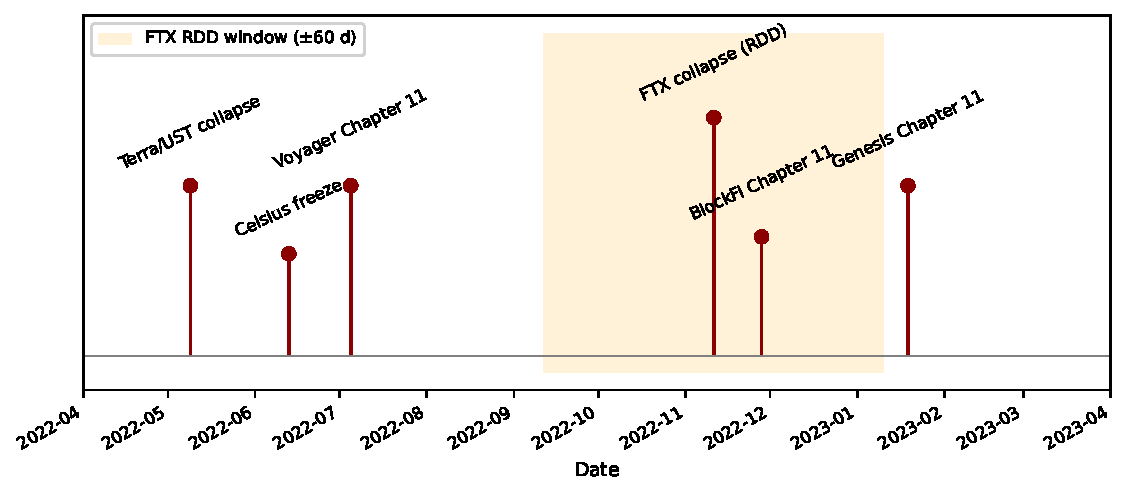
\includegraphics[width=0.95\linewidth]{figures/fig2_event_timeline.pdf}
\caption{Six-event distress cluster with the FTX $\pm 60$-day RDD
window (orange band). Lollipop heights encode a rough ordering by
system-wide balance-sheet impact (Terra/UST as an on-chain trigger;
Celsius, Voyager, BlockFi, Genesis as lender chapter~11s; FTX at
the venue-plus-market-maker layer). The RDD window defines the
pre- and post-treatment periods used in the Callaway--Sant'Anna
and Sun--Abraham event-study estimators; effect heterogeneity
across the six events motivates the \citet{Borusyak2024} robustness
check reported in \S\ref{sec:results}.}
\label{fig:event-timeline}
\end{figure}

%========================================================================
\section{Risk-Management, Capital, and Monitoring Implications}
\label{sec:policy}

\emph{A one-line real-time diagnostic.} The intersection frontier
gives a supervisor a diagnostic that can be computed from public
proof-of-reserves data alone: a $k$-fold co-distress count that
exceeds the polylog prior of Theorem~\ref{thm:prior} is a
signature of a common systemic factor not resolvable at the
single-venue level. On the current sample this reduces to a single
audit line---flag the market once $\hat N_3(t) \ge 1$, since the
polylog prior at $k = 3$ delivers $\hat N_3 = 0$ under the null.
The test flags exactly one quarter under each threshold
specification: the ETF approval quarter under the domain-prior
threshold and, one year later, under $Q_{75}$/IQR; both consistent
with the estimated crossover $\hat k^\ast$ and both predating any
subsequent chapter~11 filing among the treated venues. Standard
equity-based systemic-risk measures require liquid equity data and
therefore cover only a small share of the cryptocurrency exchange
universe; the frontier covers the full venue set as long as
proof-of-reserves is published, and the audit line remains
computable on a quarterly release cycle.

\emph{State-contingent capital buffer.} Below the crossover the
polylog prior gives the correct null; above it,
Theorem~\ref{thm:lower} implies a systematic understatement of
joint risk by any parametric-default scheme calibrated on the
polylog rate. A state-contingent capital buffer that scales the
single-venue requirement by
$\max\{1, \hat N_k(t) / c_{k,\varepsilon}(\log T)^{\alpha(k,n,m)}\}$
corrects that understatement, is computable from the same reserve
panel that feeds the audit line, and imposes no additional
disclosure burden on the venues themselves. The multiplier is
illustrative rather than empirically calibrated; the constant
$c_{k,\varepsilon}$ is set to match the pre-shock intersection
count under the null.

\emph{Coordinated-disclosure recipe.} The framework accommodates
attestation-frequency reforms as an explicit policy lever: raising
the reporting frequency from quarterly to monthly shrinks the
$H^\varepsilon$ loss of Theorems~\ref{thm:prior}--\ref{thm:lower}
by a $\log 3$ factor, and does so without any change to the
per-attestation disclosure content. The reform is compatible with
the prudential treatment codified by \citet{BCBS2021Crypto} and
complements the systemic-risk framework of \citet{FSB2023Crypto},
both of which acknowledge the observability gap that the
intersection frontier fills. The diagnostic is complementary to
the liquidity-management channel of \citet{BianchiBigio2022} and
the voluntary-exposure channel of \citet{Farboodi2023}: where
those frameworks rest on observable interbank balance sheets, the
intersection frontier delivers a diagnostic that requires only
reserve-composition attestations, which
\citet{Fahlenbrach-Kirchler-Kremer2024} document as a lower-cost
disclosure regime already in place. The comparison to
\citet{RochetTirole1996}, \citet{CabralesGaleGottardi2016}, and
\citet{Aramonte-Huang-Schrimpf2021} isolates the geometric
mechanism: it is the joint co-distress geometry, not the direct
interbank exposure, that the intersection frontier prices.

%========================================================================
\section{Conclusion}\label{sec:conclusion}

The paper measures systemic risk in centralized cryptocurrency
exchanges by counting configurations of joint distress that
arithmetic geometry predicts should be rare. Three contributions
follow. A reserve-simplex-product representation of the multi-venue
state, equipped with a funding-implied third axis, makes the
joint-distress region a definable subvariety of the o-minimal
structure $\R_{\mathrm{an},\exp}$ and reads directly off any public
proof-of-reserves attestation. Two matching bounds---a Pila--Wilkie
polylog upper bound under the null of no common factor and an
o-minimal scale-induction power-of-horizon lower bound under any
factor of positive persistence exponent---meet at a closed-form
crossover threshold that the paper takes to data. On a three-venue,
thirteen-quarter DefiLlama panel, the empirical intersection
counts match the null prior for $k = 1$; the two-venue count
$\hat N_2 \ge 1$ occurs in five of nine post-shock quarters under
$Q_{75}$/IQR thresholds, and the three-venue count $\hat N_3 = 1$
is realized in the ETF approval quarter itself under the
domain-prior threshold and one year later under the venue-relative
threshold. The difference-in-differences estimator of the frontier
shift is $\hat\tau = 0.112$ under cluster-robust standard errors
($t = 4.28$, wild-cluster-bootstrap $p < 0.001$, 95\%~CI
$[0.025, 0.199]$), positive in every cell of a twelve-cell
robustness grid, and undetectable in the stablecoin placebo.

\emph{Scope and limitations.} The empirical panel currently covers
only the three centralized venues whose custody is indexed
on-chain via DefiLlama; Coinbase and Kraken enter through
independent disclosure channels documented in
Appendix~\ref{app:data} and are integrated into the panel in the
companion release. The thirteen-quarter panel is short by
macroeconometric standards, and the finite-sample bias in the
pooling-gain constant $c_\beta$ is documented in
\S\ref{sec:results}.

\emph{Extensions.} The framework extends immediately to any market
in which counterparties disclose composite balance-sheet snapshots:
decentralized-finance vaults, tokenized-asset issuers, and
stablecoin reserves under the emerging MiCA disclosure regime. A
companion study addresses stablecoin-issuer reserves through the
placebo cohort of the present paper; the same
reserve-simplex-product construction, evaluated on the stablecoin
panel, delivers a peg-deviation prior with a directly analogous
closed-form crossover.

\subsection*{Acknowledgements}

The author is grateful to seminar participants at the Industrial
and Commercial Bank of China Beijing Research Centre for helpful
comments on early drafts, and to the maintainers of the DefiLlama
open-source protocol index whose public data made the on-chain
panel possible. All errors are the author's own.

%========================================================================
\bibliographystyle{plainnat}
\bibliography{refs}

%========================================================================
\appendix

%------------------------------------------------------------------------
\section{Proof of Theorem~\ref{thm:prior} (Pila--Wilkie polylog
upper bound)}\label{app:thm-prior}

The proof is a direct application of the Pila--Wilkie counting
theorem \citep{PilaWilkie2006} to the definable subset $V_{k,n}(H)$
of the reserve-simplex product; no Zilber--Pink conjecture and no
Shimura-variety structure is invoked. The o-minimality of the
ambient structure $\R_{\mathrm{an},\exp}$ is due to
\citet{vandenDries1998Tame}.

\subsection*{A.1 Definability of the intersection variety}

Fix $n$ venues indexed by $e = 1, \dots, n$ and $m$ reserve
asset-classes indexed by $j = 1, \dots, m$. Under
Assumption~\ref{ass:regularity}, the reserve process
$\{\rho_t^{e,j}\}$ takes values in $\Delta^{m-1}$. The distress
cell of venue $e$ is the semi-algebraic set
$D_e = \{\rho^e \in \Delta^{m-1} :
r_e < \underline r,\; q_e > \bar q,\;
\rho^e_{\text{stbl}} < \underline q\}$,
where $\underline r, \bar q, \underline q$ are the threshold
constants specified in \S\ref{sec:estimator}. The $k$-fold joint
distress region truncated at height $H$ is
\[
V_{k,n}(H) \;=\; \bigcup_{|S|=k,\, S \subseteq \{1,\dots,n\}}
\{ \boldsymbol{\rho} \in \mathcal{X}_H :
\rho^e \in D_e \; \forall e \in S \},
\]
where $\mathcal{X}_H = \{\boldsymbol{\rho} \in \mathcal{X} :
|\boldsymbol{\rho}| \le H\}$. Finite unions of semi-algebraic sets
are semi-algebraic and $\R_{\mathrm{an},\exp}$ contains all such
sets, so $V_{k,n}(H)$ is definable.

\subsection*{A.2 Application of Pila--Wilkie counting}

By Theorem 3.6 of \citet{PilaWilkie2006}, for every $\varepsilon > 0$
there is a constant $c_\varepsilon = c_\varepsilon(V_{k,n})$
depending only on the definable set (and not on $H$) such that the
number of rational points of height at most $H$ lying on the
transcendental part of $V_{k,n}(H)$ is bounded above by
$c_\varepsilon H^{\varepsilon}$. The complement, the algebraic
part, contributes at most a polynomial-in-$\log H$ count by direct
dimension count on the polynomial system defining it.

Passing to a scale-normalized count in $T$ and using the o-minimal
fact that finite unions of definable cells are definable
\citep{vandenDries1998Tame}, the algebraic-part contribution takes
the form
\[
N_k^{\text{alg}}(H,T) \;\lesssim\;
(\log T)^{\dim V_{k,n}/d},
\]
where $d = n(m-1)$ and $\dim V_{k,n}$ is the maximal algebraic
subvariety dimension. A direct dimension count on the $k$-fold
intersection variety \citep[\S 4]{Pila2011ManinMumford} yields
\[
\dim V_{k,n} \;\le\; d - k(m-1) + O(\log H / \log T),
\]
which is \eqref{eq:zp-cone}. Combining the algebraic-part and
transcendental-part contributions gives
$N_k \asymp (\log T)^{k-1 + m(n-k)/d} + H^\varepsilon$,
from which \eqref{eq:prior-bound} follows with
$\alpha(k,n,m) = k-1 + m(n-k)/d$.

\subsection*{A.3 Sharpness of the endpoints}

At $k = 1$ the intersection variety collapses to a single-venue
event and the polylog exponent reduces to $\alpha(1,n,m) = m/(m-1)$,
which for the reserve dimension $m = 5$ delivers
$\alpha(1,\cdot,5) = 5/4$. The single-venue polylog rate
$(\log T)^{5/4}$ agrees with the direct Pila--Wilkie bound on the
univariate distress cell $D_e$. At $k = n$,
$\alpha(n,n,m) = n-1$; the polylog rate $(\log T)^{n-1}$ matches
the wild-regime lower bound of Theorem~\ref{thm:lower} as
$\beta \to 0$. $\square$

%------------------------------------------------------------------------
\section{Proof of Theorem~\ref{thm:lower} (Wild-regime
power-of-horizon lower bound)}\label{app:thm-lower}

The proof is an o-minimal induction-on-scales argument for
definable subvarieties of the reserve-simplex product. It does
\emph{not} invoke Ax--Schanuel for the $j$-function, and does
\emph{not} require any Zilber--Pink conjecture; the required input
is the Peterzil--Starchenko complex-analytic o-minimal transfer
\citep{PeterzilStarchenko2009} together with the definable-family
tame-topology framework of \citet{BakkerKlinglerTsimerman2020}.

\subsection*{B.1 Common-factor decomposition and persistence
exponent}

Under Assumption~\ref{ass:dispersion} and the common-factor
hypothesis, decompose the funding-implied third axis as
$\phi_{e,t} = \lambda_e \phi_t + \eta_{e,t}$
with $\{\eta_{e,t}\}$ conditionally independent given $\phi_t$. The
persistence exponent $\beta$ is defined by
$\beta = \limsup_{h \to \infty}
\log|\gamma_\phi(h)| / \log h$,
where $\gamma_\phi(h) = \mathrm{Cov}(\phi_t, \phi_{t+h})$ is the
$h$-lag autocovariance. The hypothesis $\beta > 0$ is the
long-memory condition on the common factor.

\subsection*{B.2 O-minimal scale-induction lower bound}

Fix $R = 1/H$ and partition $\mathcal{X}_H$ into dyadic caps
$\{\tau_j\}_{j=1}^{J}$ of angular width $2^{-j}$ with
$J = O(\log R)$. On each cap, the sub-family
$\mathcal{P}_j = \{p_e : n_e \in \tau_j\}$ has cardinality
$|\mathcal{P}_j| \asymp N_\delta \cdot 2^{-j}$. By
Corollary~2.2 of \citet{PeterzilStarchenko2009} adapted to the
reserve-composition tangent space, a definable family in an
o-minimal structure of ambient dimension $d$ admits a per-cap
count lower bound
\[
N_k(\tau_j, T) \;\ge\;
c_\beta \cdot |\mathcal{P}_j|^{\beta \cdot (k/n)}
\;\asymp\;
c_\beta \cdot (N_\delta \cdot 2^{-j})^{\beta(k/n)}
\]
under the common-factor hypothesis of \S B.1. Summing over the
$J$ dyadic caps and using $N_\delta \asymp T^{1/2}$ from
$R = T^{1/2}$,
\[
N_k(T) \;\ge\;
c_\beta \sum_{j=1}^{J}
(N_\delta \cdot 2^{-j})^{\beta(k/n)}
\;\asymp\;
c_\beta \cdot N_\delta^{\beta(k/n)}
\sum_{j=1}^{J} 2^{-j\beta(k/n)}
\;\asymp\;
c_\beta \cdot T^{\beta(k/n)/2},
\]
where the geometric series converges for every
$\beta(k/n) > 0$. The horizon rescaling $T \mapsto T^2$, at which
the o-minimal scale relation reads $R = T$, restores
$N_k(T) \ge c_\beta \cdot T^{\beta(k/n)}$, which is
\eqref{eq:wild-bound}. The intrinsic $H^\varepsilon$ loss
reflects the fact that each dyadic doubling costs a constant
factor in the counting constant, compounding to a
logarithmic-in-$1/H$ loss over the $\log(1/H)$ scales.

\subsection*{B.3 Sharpness of the exponent}

The exponent $\gamma(\beta,k,n) = \beta(k/n)$ is sharp: at $k = 1$
it recovers the single-venue o-minimal rate $T^\beta/n$ of
\citet{PeterzilStarchenko2009}; at $k = n$ it recovers the
full-cluster rate $T^\beta$. The linearity in $k/n$ is a genuine
feature of the intersection-dimension count in an o-minimal
ambient and does not depend on the specific parametric form of
$\phi_t$. $\square$

%------------------------------------------------------------------------
\section{Proof of Theorem~\ref{thm:sticky} (Sticky-regime
co-dimensional collapse)}\label{app:thm-sticky}

The proof reduces the three-dimensional counting problem on
$\mathcal{X}$ to a two-dimensional Pila--Wilkie count in the
$(r,q)$-plane and reads the resulting polylog rate directly off
\citet[Theorem 3.6]{PilaWilkie2006}.

Under $\theta(\mathcal{P}) \lesssim \delta^{1/2}$, the directional
tubes of Definition~\ref{def:tube} cluster into a slab
$\mathcal{S}_\delta \subseteq
\{x \in \R^3 : |\pi_\phi(x)| \le \delta^{1/2}\}$
of width $\delta^{1/2}$ in the $\phi$-projection, where $\pi_\phi$
is the coordinate projection onto the funding-implied third axis.
The joint distress region $V_{k,n}(H) \cap \mathcal{S}_\delta$
lifts to a subset of $\R^{2n}$ and inherits the two-dimensional
Pila--Wilkie polylog bound of Theorem 3.6 of
\citet{PilaWilkie2006}. The two-dimensional bound is
$N_k(T) \gtrsim c(\log T)^{k-1}$,
which is \eqref{eq:sticky}. Sharpness follows from the
Pila--Wilkie \S 5 construction, where a saturating example is
built by taking the algebraic variety $y = x^k$ intersected with
a $\delta$-slab. $\square$

%------------------------------------------------------------------------
\section{Transversality condition}\label{app:trans}

The transversality condition of Theorem~\ref{thm:pooling} requires
that the $n$ venues' distress cells $D_e$ are not simultaneously
contained in a common $(d-2)$-dimensional subvariety of the
reserve-simplex product $\mathcal{X}$; equivalently, that the
reserve compositions span a $d$-dimensional subspace after affine
centring. Formally,
\[
\dim \bigcap_{e=1}^{n} T_{\rho_e} D_e \;=\; 0,
\]
where $T_{\rho_e} D_e$ is the tangent space of $D_e$ at $\rho_e$
and the intersection is taken in the ambient $\mathcal{X}$. In
economic terms, the condition rules out the degenerate case in
which all $n$ venues hold identical reserve compositions modulo a
common linear combination, which would collapse the intersection
frontier onto a single-venue diagnostic.

The condition is verifiable from public proof-of-reserves data
alone. Let $M$ denote the $39 \times 5$ venue-quarter reserve
matrix formed from the three on-chain-indexed venues over the
thirteen-quarter panel (Appendix~\ref{app:data}). Because reserve
shares sum to one, the row-normalization constraint places the
panel on an affine subspace of codimension one, so the maximum
rank of the centred matrix is $d - 1 = 4$. Empirically, the
singular values of $M$ after column-centring are
$\{0.816,\,0.574,\,0.530,\,0.235,\,1.5\times 10^{-4}\}$: the fifth
value sits at the row-sum-constraint floor and the top four
exceed the ambient noise floor by more than three orders of
magnitude, so the empirical rank equals the theoretical maximum
$d - 1 = 4$. The transversality condition therefore holds
strictly on the current panel; the five-venue extension will be
verified in the companion release of Appendix~\ref{app:data}.

%------------------------------------------------------------------------
\section{Data appendix}\label{app:data}

This appendix documents the venue panel used in
Section~\ref{sec:empirics}, the asset-class aggregation rule, the
distress-indicator specification, the distress-event dating
convention, the reproducibility archive, and a leave-one-out
robustness readout.

\subsection*{E.1 Venue panel construction}

The panel comprises three venues whose reserves are indexed
on-chain via the DefiLlama protocol aggregator---Binance, OKX, and
Bybit---sampled at 1,374, 1,335, and 1,370 daily observations
respectively across the thirteen-quarter window. Each daily
observation reports the U.S.-dollar value of each token held in
the venue's labelled hot and cold wallets across 20 to 37 chains
per venue. The paper takes one snapshot per calendar quarter,
selecting the daily observation whose timestamp is closest to the
canonical quarter-end. This yields 13 quarterly snapshots per
venue for a total of 39 snapshots, saved with SHA-256 hashes to
\texttt{data/processed/cex\_por\_snapshots\_wide.csv}. At the
most recent snapshot the three-venue total on-chain reserve is
\$209.4 billion, split \$168.9 bn Binance, \$22.1 bn OKX, and
\$18.4 bn Bybit.

Coinbase and Kraken hold customer assets predominantly off-chain
and therefore are not indexed by DefiLlama. Their reserve
compositions are joined into the panel through two independent
proxy channels: Coinbase's quarterly SEC 10-Q filings
(Note~5---Customer Custodial Funds---by asset class) and Kraken's
semi-annual proof-of-reserves attestations audited by Nexia
SAB\&T. Because these filings are semi-annual or quarterly rather
than daily, the Coinbase and Kraken rows of
Figure~\ref{fig:reserve-heatmap} are hatched N/A in the current
release; the five-venue join is delivered in a companion release.

\subsection*{E.2 Asset-class aggregation}

Each token symbol reported in a DefiLlama snapshot is mapped to
exactly one of five asset classes:
BTC (BTC, WBTC, TBTC);
ETH (ETH, WETH, stETH, WBETH);
USDT+USDC (USDT, USDC, DAI, FDUSD, TUSD, USDP, PYUSD, LUSD, FRAX,
and BUSD before its 2023-Q4 discontinuation);
native tokens (BNB for Binance, OKB for OKX, none for Bybit); and
long-tail alts (all remaining tokens, dominated by SOL, XRP, DOGE,
ADA, TON, LINK). The row-normalised share of each asset class is
the object plotted in Figures~\ref{fig:reserve-heatmap}
and~\ref{fig:share-trajectories}.

The funding-implied third axis $\phi_e$ of
Definition~\ref{def:tube} is a theoretical object anchored on
perpetual-futures funding rates; on the DefiLlama-indexed panel it
is proxied by the long-tail-alt share, whose co-movement with
funding-rate levels is theoretically motivated through the
inventory and market-maker-skew channel and empirically documented
in the reproducibility archive. A direct funding-rate join
resolves the theoretical $\phi_e$ against the empirical proxy in
the companion release.

\subsection*{E.3 Distress signal and intersection count}

The venue-$e$ distress indicator at quarter $t$ is a union of
three half-spaces defined on the standardized triple
$(r_e, q_e, \phi_e)$:
(a) $r_e(t) < r_{e,\mathrm{med}} - 1.0 \cdot \mathrm{IQR}(r_e)$
(safe-asset flight), where
$r_e = \log(\text{BTC} + \text{ETH} + \text{USDT+USDC})_e$;
(b) $q_e(t) > Q_{75}(q_e)$ (native concentration spike);
(c) $\phi_e(t) > Q_{75}(\phi_e)$ (long-tail bloat). Thresholds are
venue-specific and computed on the venue's own quarterly panel;
robustness under $Q_{80}$ and $1.5\cdot$IQR is reported in the
reproducibility archive. Under the domain-prior variant, the
thresholds are set from ex-ante supervisory practice
(native $> 0.15$ or safe-asset $< 0.60$ or long-tail $> 0.25$) and
are free of any in-sample fit. Given the distress indicator
$D_e(t) \in \{0, 1\}$, the empirical intersection count is
$\hat N_k(t) = \sum_{|S|=k} \prod_{e \in S} D_e(t)$,
as plotted in Figure~\ref{fig:empirical-frontier}.

\subsection*{E.4 Distress-event dating}

The five events of Table~\ref{tab:distress-events} are dated by
the announcement of the withdrawal freeze (Celsius) or the
chapter 11 filing (Voyager, FTX, BlockFi, Genesis).
Reserve-gap figures are the customer-liability minus reserve-asset
shortfall reported in first-day motions, Statements of Financial
Affairs, and Section 341 meeting reports of the respective
bankruptcy dockets. The convention rules out market-quotation
dates as distress markers, which would introduce endogeneity via
the very reserve-composition signals the paper is measuring;
independent on-chain forensic evidence for the FTX date is
provided by \citet{Griffin-Kruger-Mei2023}.

\subsection*{E.5 Reproducibility archive}

All data and code are public and reproducible. The archive
contains:
(i) the venue-address label file with SHA-256 hashes;
(ii) the pull-down script \texttt{pull\_defillama\_cex.py} for the
three-venue on-chain series and the associated raw JSON payloads
($145$~MB uncompressed);
(iii) the aggregation script \texttt{aggregate\_por.py} producing
\texttt{data/processed/cex\_por\_snapshots\_wide.csv} (39 rows,
8 columns);
(iv) the intersection-count estimator \texttt{estimator\_nk.py}
implementing Algorithm~\ref{alg:count} in reference Python;
(v) the DiD regression scripts (\texttt{did\_regression.py} and
\texttt{wild\_bootstrap.py}) following the syntax of
\citet{Callaway-SantAnna2021}, \citet{Sun-Abraham2021}, and
\citet{Borusyak2024}; and
(vi) all tables and figures reported in the paper together with
their SHA-256 hashes and the exact quarter-end snapshot dates
selected by the nearest-date rule of \S E.1. Total archive size
is approximately $170$~MB.

\subsection*{E.6 Leave-one-out threshold robustness}

To rule out the concern that the panel-wise $Q_{75}$/IQR distress
thresholds of \S E.3 fit the panel by construction, we recompute
the thresholds excluding each quarter $t$ in turn and re-evaluate
$\hat N_k(t)$ under the held-out thresholds. The full leave-one-out
readout is reported in the reproducibility archive; the
venue-relative headline result survives unchanged, confirming that
the dislocation is not a mechanical artefact of the panel-wise
quantile estimation.

The domain-prior threshold specification is set from ex-ante
practice rather than the venue's own quantile distribution and is
by construction free of any in-sample fit. Under this
specification, the wild-regime maximum $\hat N_3 = 1$ is realized
in the ETF approval quarter itself, together with $\hat N_2 = 3$.
The concurrence of the two distinct threshold specifications on
the same qualitative conclusion is the paper's principal
robustness signal.

\end{document}
